%===============================================================================
\section{Project information}
\label{section:project_information}

% Project
This paper covers the project plan for the the project Multi-robot Soccer - RoboCup. This project is a collaboration with \ac{udea} and \ac{utp}. The project consists of developing both the hardware and the software for one \ac{ssl}-RoboCup division B robot. The project will assume and follow Swedish laws and standards, unless the \ac{ssl}-RoboCup rules explicitly requires otherwise. When neither is available or ambiguous, the project will refer to European laws and standards.
% Contributors
The project team consists of eleven contributors split into a hardware and a software team, see Table.\:\ref{tab:contributors_roles}. 
% Software
The software team was further divided into communication, individual robot behaviour and collective robot behaviour. Collective robot behaviour is tasked with deciding the overarching strategy and tactics for the entire robot team. Individual robot behaviour is charged with finding a suitable way to execute the desired behaviour from the perspective of an individual robot. Communication involves simulation and \ac{ssl} interfacing, as well as peer to peer communication. See Fig.\:\ref{fig:software_structure} for a visual understanding of how the different modules connect.
% Hardware
The hardware team was split into four groups: powertrain \& electronics, sensors \& embedded systems, 3D-\acs{cad} \& body design and mechanical design. Powertrain \& electronics designs and implements the power system for the robot including batteries, motors, \ac{esc} and the dribbler. Sensors \& embedded systems integrates the sensors and processes the data. 3D-\acs{cad} develops the chassis and all 3D modelling requirements. Mechanical design develops the kicker system.

\begin{table}
    \centering
    \resizebox{\columnwidth}{!}{\noindent\begin{tabular}{|c|c|c|} \hline
         \textbf{Name}          & \textbf{Role}                                         & \textbf{Task}                                 \\ \hline
         Viktor Eriksson        & Software developer                                    & Collective robot behaviour                    \\ \hline
         Anton Grusell          & Hardware developer                                    & 3D-\acs{cad} \& Body design                   \\ \hline
         Mudar Ibrahim          & Team leader \& Software developer                     & Communication                                 \\ \hline
         Jacob Johanssson       & Software developer                                    & Collective robot behaviour                    \\ \hline
         Aaiza Aziz Khan        & Software developer                                    & Communication                                 \\ \hline
         Carl Larsson           & Software lead \& Software developer                   & Individual robot behaviour                    \\ \hline
         Johanna Melander       & Hardware developer                                    & Mechanical design                             \\ \hline
         Shruti Puthiya Kunnon  & Software developer                                    & Communication                                 \\ \hline
         Pontus Svensson        & Team leader \& Hardware lead \& Hardware developer    & Power-train \& Electronics                    \\ \hline
         Fredrik Westerbom      & Hardware developer                                    & Sensors \& Hardware communication             \\ \hline
         Emil Åberg             & Software developer                                    & Individual robot behaviour \& Communication   \\ \hline
    \end{tabular}}
    \caption{Project contributors, including their roles and assigned tasks.}
    \label{tab:contributors_roles}
\end{table}

\begin{figure}
    \centering
    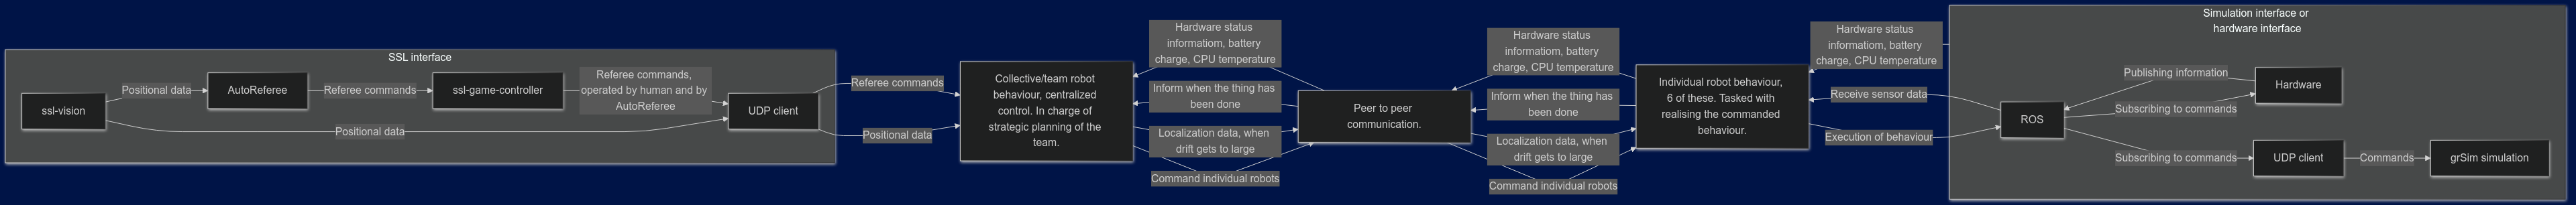
\includegraphics[width=\linewidth]{images/DVA490_software_structure.png}
    \caption{Software structure describing the interaction and connection between the different software modules.}
    \label{fig:software_structure}
\end{figure}

%===============================================================================